\chapter{Functional Safety}
\section{Introduction and Objectives}
The hand exoskeleton under development in this thesis is intended for direct physical interaction with the human body. In such a scenario, any malfunction in the sensing, actuation, or control software may result in unintended forces or motions applied to the user's fingers, with potential consequences ranging from discomfort to physical injury. Functional safety is therefore not an optional feature but a core design requirement that must be addressed at every level of the system architecture.
 
The control framework described in Chapter 4 already incorporates several point-wise safety provisions, including torque saturation at the trajectory controller output (Equation 4.16), velocity and position clamping in the admittance loop (Section 4.2.3), and joint position bounds enforced on the virtual coordinate. While these mechanisms are effective under nominal operating conditions, they do not address the broader class of faults that can arise in a distributed ROS 2 architecture: a crashed node, a stale sensor measurement, a corrupted control signal, or a mismatch between the commanded and actual operating mode of the system.

This chapter presents the dedicated \textbf{functional safety layer} that was developed as part of the Digital Twin to address these concerns. The design follows a \textbf{defense-in-depth} philosophy, in which multiple independent mechanisms cooperate to detect, classify, and mitigate fault conditions before they can propagate to the actuator and ultimately to the user. Rather than relying on a single centralized monitor, the architecture distributes safety responsibilities across several specialized nodes, each operating at a different level of abstraction and capable of triggering protective actions autonomously.

The functional safety layer is implemented across four ROS 2 packages within the Digital Twin workspace:

\begin{itemize}
    \item \textbf{exoskeletron\_safety\_manager}: a C++ state machine that governs the overall safety state of the system through a plugin-based architecture, manages transitions between operating modes, and coordinates the response to detected faults;
    \item \textbf{exoskeletron\_safety\_msgs}: custom ROS 2 message and service definitions that provide a structured communication interface for the safety subsystem;
    \item \textbf{exoskeletron\_supervision}: the `ExoBridge` node, a safety-enforcement gateway that mediates all control signals between the controllers and the dynamic plant, physically enforcing torque limits, velocity bounds, and stop conditions;
    \item \textbf{exoskeletron\_faults}: a fault injection framework for the systematic validation of the safety mechanisms under controlled and reproducible fault scenarios.
\end{itemize}

The architecture is designed to be \textbf{extensible}: each safety mode is implemented as a dynamically loadable plugin through the ROS 2 `pluginlib` framework, allowing new modes to be added without modifying the state machine core. All safety thresholds, watchdog timeouts, and debounce parameters are exposed as ROS 2 parameters and can be tuned at launch time through a dedicated configuration file (safety\_params.yaml), without recompilation.

The remainder of this chapter describes the safety architecture in detail. Section 5.2 provides an overview of the three-layer structure. Section 5.3 presents the safety state machine and its transition logic. Section 5.4 describes the fault detection and escalation mechanism implemented in the `FaultMonitorMode` plugin. Section 5.5 discusses the `ExoBridge` enforcement node, including its per-channel watchdog system and the bridge supervision performed by the state machine. Section 5.6 covers the automatic downgrade mechanism. Section 5.7 documents the custom safety messages. Section 5.8 presents the fault injection framework used for validation. Finally, Section 5.9 summarizes the chapter. The observer-based fault detection approach, which provides an additional model-based detection channel, is briefly discussed in the following chapter.

\section{Safety Architecture Overview}
The functional safety architecture of the Digital Twin is organized into three logically distinct layers, each responsible for a specific aspect of the safety function. This separation ensures that no single node is simultaneously responsible for detecting a fault and enforcing the corrective action, a principle that is central to the design of safety-critical systems.

\subsection{Three-Layer Structure}
The three layers operate at different levels of abstraction within the ROS 2 node graph and are connected through a well-defined set of topics and services. Their roles can be summarized as follows.

The \textbf{enforcement layer} is implemented by the ExoBridge node (package \textbf{exoskeletron\_supervision}). This node sits on the data path between the control nodes described in Chapter 4 and the dynamic plant described in Chapter 3. Every torque command and trajectory reference passes through the bridge before reaching the plant. Depending on the active safety mode, the bridge applies torque clamping, velocity and acceleration limiting, or complete torque zeroing (safe stop). The bridge also maintains independent per-channel watchdogs on the four critical input signals - torque command, trajectory reference, external force estimate, and joint state feedback - and autonomously triggers a safe stop request if any of these signals becomes stale. The enforcement layer is therefore capable of protecting the user even in the absence of higher-level supervision, providing a last line of defense against undetected faults.

The \textbf{detection and escalation layer} is implemented by the \textbf{FaultMonitorMode} plugin within the \textbf{exoskeletron\_safety\_manager} package. When the state machine is in its nominal operating state (\textbf{FAULT\_MONITOR}), this plugin subscribes to the bridge status topic and continuously evaluates the actual torque delivered to the plant and the crank angular velocity against a set of configurable thresholds. The evaluation follows a multi-level escalation logic: depending on the severity of the detected anomaly, the monitor requests a transition to \textbf{COMPLIANT\_MODE}, \textbf{TORQUE\_LIMIT\_MODE}, or \textbf{SAFE\_STOP}. A debounce mechanism based on per-level sample counters prevents spurious escalation due to transient peaks or measurement noise.

The \textbf{governance layer} is implemented by the \textbf{StateMachine} node, the central coordinator of the safety subsystem. The state machine maintains the current safety state, enforces the allowed transition graph, manages the fault latching mechanism for the SAFE\_STOP state, and coordinates the bridge operating mode through an asynchronous service interface. It also performs two additional supervision tasks on the bridge itself: a liveness check that verifies the periodic reception of bridge status messages, and a mode coherence check that compares the operating mode reported by the bridge with the mode expected by the state machine. A sustained mismatch in either check triggers an automatic transition to SAFE\_STOP.

Figure 5.1 illustrates the overall architecture, showing the three layers, the ROS 2 topics and services connecting them, and the position of the safety subsystem relative to the control and plant nodes described in the preceding chapters.

\afterpage{
\begin{sidewaysfigure}
\centering
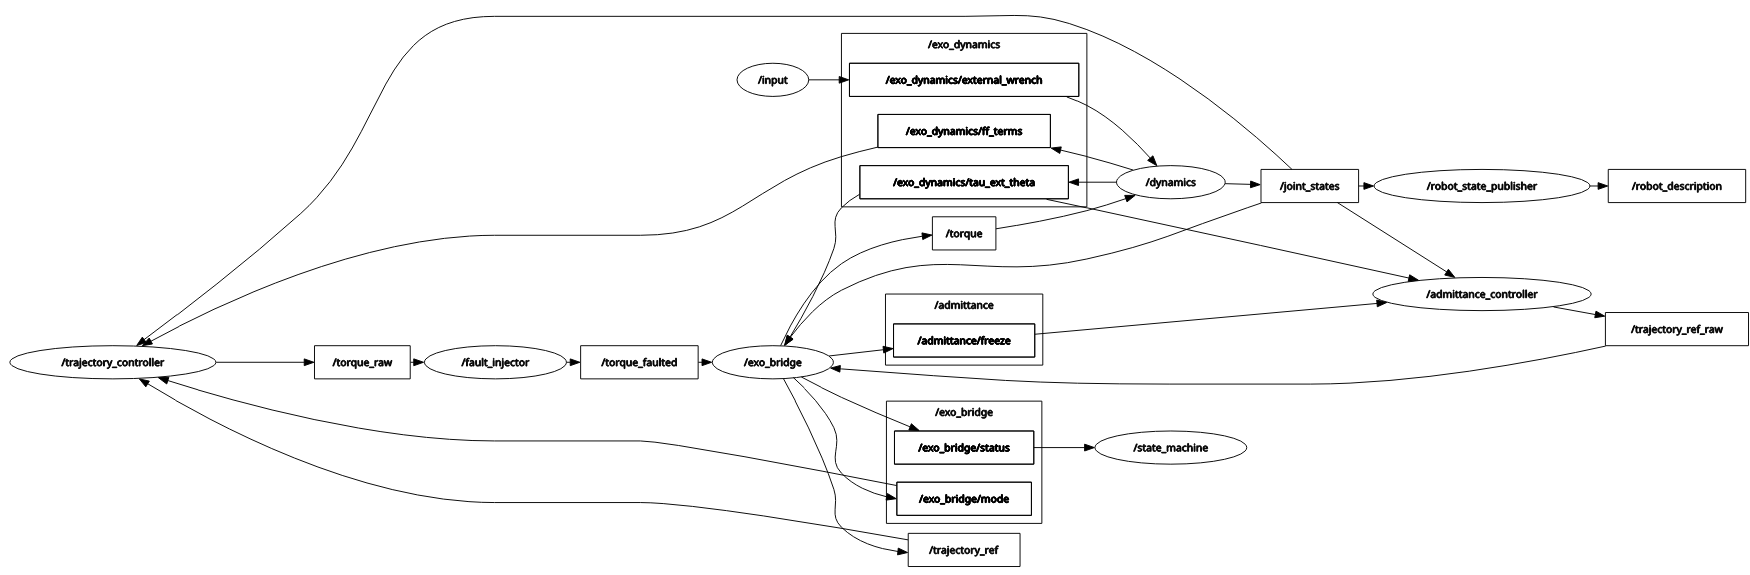
\includegraphics[width=\textheight]{images/chapter5/rosgraph_completo2_ch5_migliore.png}
\label{fig:rosgraph_completo}
\caption{Functional Safety Architecture: ROS 2 Node Graph}
\end{sidewaysfigure}
\clearpage
}




\subsection{Plugin-Based Design}
A distinctive feature of the safety architecture is the use of the ROS 2 pluginlib framework to implement the individual safety modes as dynamically loadable plugins. All safety modes inherit from a common abstract base class, \textbf{SafetyTools}, which defines the lifecycle interface that each plugin must implement:

\begin{minted}{cpp}

    class SafetyTools
    {
    public:
    virtual void initialize(const rclcpp::Node::SharedPtr & node) = 0;
    virtual void stop() = 0;
    virtual void pause() = 0;
    virtual void resume() = 0;
    virtual void shutdown() = 0;
    virtual void set_safety_params(double param) = 0;
    };

\end{minted}

The \textbf{initialize()} method receives a shared pointer to the state machine node itself, allowing each plugin to create its own subscribers, service clients, and timers on the same node handle. This design avoids the overhead of additional node instances while preserving modularity. The \textbf{stop()} and \textbf{resume()} methods provide hooks for pausing and restarting the plugin's activity during state transitions, and \textbf{shutdown()} releases all ROS 2 resources created by the plugin.

Each plugin that needs to communicate an operating mode to the \textbf{ExoBridge} inherits from a second base class, \textbf{BridgeModeClient}, which provides a reusable asynchronous service client for the \textbf{/bridge/set\_mode service}. The BridgeModeClient includes response verification logic: upon receiving the service response, it logs whether the bridge accepted or rejected the mode change and tracks the last confirmed mode. This design ensures that every mode transition is explicitly confirmed by the bridge, rather than assumed.

The plugin architecture allows the safety subsystem to be extended with new safety modes - for example, a future \textbf{SensorDegradedMode} for operation with partial sensor availability - without modifying the state machine code. The mapping between safety states and plugin class names is maintained within the state machine and exposed through the \textbf{state\_to\_plugin\_name()} method. The plugin discovery and instantiation is handled entirely by \textbf{pluginlib} at runtime, based on a \textbf{plugins.xml} descriptor file shipped with the package.

\subsection{Configuration and Parameterization}
All safety-related thresholds, timeouts, and behavioral parameters are declared as ROS 2 parameters on the state machine node and loaded from a dedicated YAML configuration file (\textbf{safety\_params.yaml}) at launch time. This approach ensures that the safety behavior can be tuned for different deployment scenarios - for instance, tighter thresholds during early-stage testing and relaxed values after a long operational period - without requiring recompilation of the C++ code.

The configuration file is organized into logical groups covering: torque and velocity thresholds for fault escalation, debounce counters for both escalation and downgrade, watchdog timeout durations, grace periods for post-initialization transients, and bridge liveness parameters.



\section{Safety State Machine}
The central element of the governance layer is the \textbf{StateMachine} node, implemented in C++ within the \textbf{exoskeletron\_safety\_manager} package. This node maintains the current safety state of the system, enforces the rules governing transitions between states, manages the fault latching mechanism, and coordinates the operating mode of the ExoBridge through the plugin lifecycle. It is instantiated as a standalone ROS 2 node and run in a single-threaded executor:

\begin{minted}{cpp}

int main(int argc, char ** argv)
    {
    rclcpp::init(argc, argv);
    auto node = std::make_shared<functional_safety::StateMachine>();
    node->initialize();
    rclcpp::spin(node);
    rclcpp::shutdown();
    return 0;
    }

\end{minted}

The \textbf{initialize()} method is called after construction to complete the setup of the ROS 2 interfaces - services, subscriptions, publishers, and the periodic status timer - once the node is fully registered in the executor. This two-phase initialization pattern is required because shared\_from\_this(), which is needed to pass the node handle to the plugins, is not available inside the constructor.

\subsection{Safety States}
The safety subsystem defines four operational states, encoded in a C++ scoped enumeration:

\begin{minted}{cpp}

    enum class SafetyState
    {
    FAULT_MONITOR = 0,
    COMPLIANT_MODE = 1,
    TORQUE_LIMIT_MODE = 2,
    SAFE_STOP = 3
    };

\end{minted}

Each state corresponds to a progressively more restrictive operating condition for the exoskeleton. A fifth state, \textbf{SENSOR\_DEGRADED\_MODE}, is reserved for future use and is not currently reachable through any transition path.
\textbf{FAULT\_MONITOR} is the nominal operating state. In this state, the FaultMonitorMode plugin is active and continuously monitors the system signals against the configured thresholds. The \textbf{ExoBridge} operates in nominal mode: all control signals pass through without modification, subject only to the plant-level saturations already present in the trajectory controller. This is the only state in which the system performs its intended rehabilitation function.

\textbf{COMPLIANT\_MODE} is the first level of degraded operation. It is entered when the fault monitor detects a moderate anomaly - for instance, a torque or velocity that exceeds the compliant threshold but remains below the torque-limit threshold. In this state, the bridge enforces reduced torque, velocity, and acceleration limits on the control signals. The admittance controller continues to operate, but the range of motion and the forces that the exoskeleton can exert on the user are significantly restricted. This mode is designed as a soft protective response that reduces the risk to the user while preserving partial functionality.

\textbf{TORQUE\_LIMIT\_MODE} represents a more severe degradation. It is triggered when the detected anomaly exceeds the torque-limit thresholds but does not yet warrant a full stop. The bridge applies a tighter torque clamp than in compliant mode, effectively limiting the maximum force that the actuator can deliver. This mode provides an intermediate level of protection between compliant operation and complete shutdown.
    
\textbf{SAFE\_STOP} is the most restrictive state and represents the ultimate protective action. Upon entry, the bridge immediately commands zero torque to the actuator and freezes the admittance controller, preventing any further motion of the exoskeleton. This state is \textbf{latched}: once entered, it can only be exited through an explicit operator reset via the \textbf{/reset\_safety\_request service}. The latching mechanism ensures that the system cannot autonomously resume operation after a severe fault, requiring human intervention to confirm that the fault condition has been resolved.

\subsection{Transition Logic and Allowed Transitions}
Not all transitions between safety states are permitted. The transition graph is designed to enforce two fundamental principles: (i) escalation is always allowed — the system can always move to a more restrictive state; and (ii) de-escalation is controlled — returning to a less restrictive state requires either an explicit operator command or the completion of the automatic downgrade procedure described in Section 5.6.

The allowed transitions are encoded in the \textbf{can\_transition\_to()} method:

\begin{minted}{cpp}

 bool StateMachine::can_transition_to(
  SafetyState target_state) const
{
  if (safe_stop_latched_ &&
      target_state != SafetyState::SAFE_STOP) return false;

  if (target_state == current_state_) return true;

  switch (current_state_) {
    case SafetyState::FAULT_MONITOR:
      return target_state == SafetyState::COMPLIANT_MODE    ||
             target_state == SafetyState::TORQUE_LIMIT_MODE ||
             target_state == SafetyState::SAFE_STOP;

    case SafetyState::COMPLIANT_MODE:
      return target_state == SafetyState::TORQUE_LIMIT_MODE ||
             target_state == SafetyState::SAFE_STOP         ||
             target_state == SafetyState::FAULT_MONITOR;

    case SafetyState::TORQUE_LIMIT_MODE:
      return target_state == SafetyState::SAFE_STOP         ||
             target_state == SafetyState::FAULT_MONITOR     ||
             target_state == SafetyState::COMPLIANT_MODE;

    case SafetyState::SAFE_STOP:
      return target_state == SafetyState::SAFE_STOP    ||
             target_state == SafetyState::FAULT_MONITOR;

    default: return false;
  }
}

\end{minted}

The first guard clause enforces the latch: if \textbf{SAFE\_STOP} has been latched, no transition to any other state is permitted until the latch is explicitly cleared. The switch statement then encodes the allowed transitions from each state, ensuring that escalation is always possible while de-escalation follows the defined paths. For example, from \textbf{COMPLIANT\_MODE}, the system can escalate to \textbf{TORQUE\_LIMIT\_MODE} or \textbf{SAFE\_STOP}, but can only return to \textbf{FAULT\_MONITOR} through an explicit request. This design ensures that the system cannot inadvertently return to a less restrictive state without a deliberate action, while still allowing for rapid escalation in response to detected faults.


\subsection{State Transition Mechanism}
All state transitions pass through a single entry point, the \textbf{request\_state\_change()} method:

\begin{minted}{cpp}

bool StateMachine::request_state_change(
  SafetyState target_state,
  const std::string & reason)
{
  if (transition_in_progress_) {
    RCLCPP_WARN(this->get_logger(),
      "Transition rejected: already in progress");
    return false;
  }

  if (!can_transition_to(target_state)) {
    RCLCPP_WARN(this->get_logger(),
      "Transition rejected: %s -> %s | reason=%s",
      state_to_string(current_state_).c_str(),
      state_to_string(target_state).c_str(),
      reason.c_str());
    return false;
  }

  if (target_state == SafetyState::SAFE_STOP) {
    latch_fault(reason);
  }

  reset_downgrade_counters();
  return change_state(state_to_plugin_name(target_state), reason);
}

\end{minted}

Three guards protect the transition. First, (\textbf{transition\_in\_progress\_}) ensures that only one transition can be active at any time, preventing race conditions in the single-threaded executor. Second, the transition graph validation rejects invalid transitions. Third, if the target state is \textbf{SAFE\_STOP}, the fault is latched before proceeding.

The actual transition is performed by \textbf{change\_state()}, which executes the following sequence: (i) the current plugin is stopped and its shared pointer is reset; (ii) a new plugin instance is created through the pluginlib class loader; (iii) the new plugin is initialized with the node handle, at which point it configures the bridge to the appropriate operating mode through the \textbf{/bridge/set\_mode} service; (iv) the internal state variable and diagnostic fields are updated; (v) the mode mismatch counter is reset to allow the bridge one to two cycles to update its reported mode.

An important design choice concerns the plugin lifecycle during transitions. In an earlier version of the implementation, the outgoing plugin's \textbf{shutdown()} method would send a request\_mode("nominal") command to the bridge, attempting to restore the default mode before the incoming plugin set its own mode. This caused a dangerous transient: during the brief interval between the \textbf{shutdown()} of the old plugin and the \textbf{initialize()} of the new one, the bridge would momentarily operate in nominal mode without any active safety enforcement. This bug was resolved by delegating the responsibility of setting the bridge mode exclusively to the incoming plugin's \textbf{initialize()} method. The outgoing plugin's \textbf{shutdown()} now only releases its ROS 2 resources without sending any mode command.

\subsection{Fault Latching and Reset}
The fault latching mechanism ensures that the most critical safety state cannot be autonomously cleared by the system. When \textbf{latch\_fault()} is invoked, three internal flags are set:

\begin{minted}{cpp}

void StateMachine::latch_fault(const std::string & reason)
{
    safe_stop_latched_ = true;
    fault_present_     = true;
    last_fault_reason_ = reason;
    RCLCPP_ERROR(this->get_logger(),
    "Fault latched | reason=%s", reason.c_str());
}

\end{minted}

The \textbf{safe\_stop\_latched\_} flag is the primary latch: as long as it is true, the first guard in \textbf{can\_transition\_to()} blocks every transition except re-entry into \textbf{SAFE\_STOP} itself. The \textbf{fault\_present\_} flag provides a secondary diagnostic indicator, and \textbf{last\_fault\_reason\_} records the human-readable cause of the fault for logging and GUI display.

The latch can only be cleared through the \textbf{/reset\_safety\_request} service, which is implemented as a \textbf{std\_srvs/Trigger} call. Upon invocation, the service handler first verifies that a fault is indeed present; if so, it calls clear\_fault\_state() to reset all three flags and the downgrade counters, and then requests a transition back to \textbf{FAULT\_MONITOR}:

\begin{minted}{cpp}

void StateMachine::reset_safety_callback(
  const std::shared_ptr<std_srvs::srv::Trigger::Request>,
  std::shared_ptr<std_srvs::srv::Trigger::Response> response)
{
  if (!safe_stop_latched_ && !fault_present_) {
    response->success = true;
    response->message = "No latched fault to reset";
    return;
  }

  clear_fault_state();

  const bool ok = request_state_change(
    SafetyState::FAULT_MONITOR, "reset");
  response->success = ok;
  response->message = ok ?
    "Safety reset completed, returned to FAULT_MONITOR" :
    "Fault cleared but failed to return to FAULT_MONITOR";
}

\end{minted}

This design ensures that the reset procedure passes through the standard \textbf{request\_state\_change()} path, preserving all the transition guards and logging. It also guarantees that the \textbf{FaultMonitorMode} plugin is properly re-initialized upon re-entry into \textbf{FAULT\_MONITOR}, including the re-activation of its bridge mode client, which explicitly sets the bridge back to nominal mode.

\subsection{ROS 2 Service Interface}
The state machine exposes four services for external interaction with the safety subsystem:

\begin{itemize}
    \item \textbf{/safe\_stop\_request} (\textbf{std\_srvs/SetBool}) - when called with data: true, requests an immediate transition to SAFE\_STOP with fault latching. This service can be invoked by any node in the system, including the ExoBridge watchdog and the \textbf{FaultMonitorMode} plugin.
    \item \textbf{/compliant\_mode\_request} (\textbf{std\_srvs/SetBool}) - when called with data: true, requests a transition to \textbf{COMPLIANT\_MODE}; when called with data: false, requests a return to \textbf{FAULT\_MONITOR} from \textbf{COMPLIANT\_MODE}.
    \item \textbf{/torque\_limit\_request} (\textbf{std\_srvs/SetBool}) - analogous to the compliant mode service, but for the \textbf{TORQUE\_LIMIT\_MODE} state.
    \item \textbf{/reset\_safety\_request} (\textbf{std\_srvs/Trigger}) - clears the fault latch and returns the system to \textbf{FAULT\_MONITOR}, as described above.
\end{itemize}

All service callbacks follow the \textbf{same pattern}: they validate the request, invoke \textbf{request\_state\_change()}, and return a response indicating success or failure with a descriptive message. The use of standard ROS 2 service types (SetBool, Trigger) ensures interoperability with existing ROS tools such as ros2 service call, facilitating both manual testing and integration with higher-level supervision systems.

\subsection{Periodic Status Publishing}
The state machine publishes its \textbf{diagnostic status} at a fixed rate of 10 Hz through a wall timer. Each status message, published on the \textbf{/safety\_manager/status} topic using the custom SafetyStatus message type (described in Section 5.7), contains the current state name and numeric identifier, the fault and latch flags, the last fault reason, the downgrade progress counters, and the bridge supervision diagnostics (liveness and mode coherence). A companion string-only topic (\textbf{/safety\_manager/state}) publishes just the state name for lightweight monitoring.

\begin{minted}{bash}

@myPC:.../ros2_ws$ ros2 topic echo /safety_manager/status

  - - -

stamp:
  sec: 1234567890
  nanosec: 123456789
  state: FAULT_MONITOR
  state_id: 0
  safe_stop_latched: false
  last_fault_reason: none
  automatic_downgrade_enabled: false
  counter_exit_compliant: 0
  counter_exit_torque_limit: 0
  bridge_alive: true
  bridge_mode_coherent: true
  last_transition_time:
    sec: 1234567890
    nanosec: 123456789
  last_transition_reason: init

  - - -

\end{minted}


The 10 Hz status timer also serves a dual purpose: at each tick, the state machine invokes the \textbf{check\_bridge\_liveness()} method (described in Section 5.5.4), which verifies that bridge status messages are being received within the configured timeout. This design choice avoids the need for an additional timer and ensures that the bridge liveness check runs at a predictable, fixed rate regardless of the bridge publication frequency.



\section{Fault Detection Plugin}
The \textbf{FaultMonitorMode} plugin is the primary software-based fault detection mechanism of the Digital Twin. It is active whenever the state machine is in the \textbf{FAULT\_MONITOR} state — that is, during nominal operation — and is responsible for continuously evaluating the system signals, classifying the severity of any detected anomaly, and requesting the appropriate escalation through the state machine service interface. The plugin is implemented in C++ and registered as a pluginlib plugin, allowing the state machine to instantiate it dynamically at runtime.

\subsection{Multi-Level Escalation}
The fault detection logic is built around a four-level severity classification, encoded in a dedicated enumeration:

\begin{minted}{cpp}

    enum class FaultResponseLevel
    {
    NOMINAL = 0,
    COMPLIANT = 1,
    TORQUE_LIMIT = 2,
    SAFE_STOP = 3
    };

\end{minted}

At each control cycle, the plugin receives the bridge status message (published at 200 Hz on \textbf{/exo\_bridge/status}) and extracts two key signals: the torque effectively delivered to the plant (\textbf{tau\_out}, corresponding to data[5] of the status vector) and the crank angular velocity (\textbf{theta\_dot}, data[3]). The choice of evaluating the post-clamp torque - rather than the raw torque commanded by the trajectory controller - is deliberate: the fault monitor is concerned with the force that the user is actually experiencing, not the force that the controller would like to apply. A scenario in which the bridge is clamping a dangerously high torque command is already being mitigated by the enforcement layer; the monitor's role is to detect whether the clamped output itself remains within safe bounds, or whether a further escalation is warranted.

Each signal is independently evaluated against \textbf{three threshold pairs} - one pair for each non-nominal severity level - through dedicated assessment methods:

\begin{minted}{cpp}

FaultResponseLevel FaultMonitorMode::evaluate_tau_entry(
  double tau_in) const
{
  const double abs_tau = std::abs(tau_in);
  if (abs_tau >= tau_safe_stop_threshold_)
    return FaultResponseLevel::SAFE_STOP;
  if (abs_tau >= tau_torque_limit_threshold_)
    return FaultResponseLevel::TORQUE_LIMIT;
  if (abs_tau >= tau_compliant_threshold_)
    return FaultResponseLevel::COMPLIANT;
  return FaultResponseLevel::NOMINAL;
}

\end{minted}

The velocity evaluation follows an identical structure with its own set of thresholds. The two individual assessments are then combined by taking the more severe of the two levels:

\begin{minted}{cpp}

    const auto tau_level     = evaluate_tau_entry(tau_in);
    const auto vel_level     = evaluate_velocity_entry(theta_dot);
    const auto instantaneous = max_level(tau_level, vel_level);

\end{minted}

This worst-case combination ensures that a dangerous condition in either signal dimension triggers the appropriate protective response, even if the other signal remains nominal.

A further constraint prevents redundant escalation: once the monitor has requested a given severity level, it will not request the same level again. Only transitions to a strictly more severe level are forwarded to the state machine. This is enforced by the \textbf{is\_more\_severe()} check applied before any service call:

\begin{minted}{cpp}

    if (!is_more_severe(entry_level, last_requested_level_)) {
  return;
}

\end{minted}

This mechanism ensures that the monitor does not flood the state machine with repeated requests for the same transition, which would be both wasteful and potentially disruptive during rapid signal fluctuations.

\subsection{Debounce Mechanism}
A critical concern in any threshold-based fault detection system is the \textbf{risk of spurious triggering} due to transient signal peaks, measurement noise, or short-lived dynamic effects. The FaultMonitorMode addresses this through a counter-based debounce mechanism that requires a fault condition to persist for a configurable number of consecutive samples before an escalation is requested.

Three independent counters are maintained, one for each non-nominal severity level. At each evaluation cycle, the counters are updated according to the instantaneous severity:

\begin{minted}{cpp}

void FaultMonitorMode::update_debounce_counters(
  FaultResponseLevel level)
{
  if (level >= FaultResponseLevel::COMPLIANT)
    ++compliant_counter_;
  else compliant_counter_ = 0;

  if (level >= FaultResponseLevel::TORQUE_LIMIT)
    ++torque_counter_;
  else torque_counter_ = 0;

  if (level >= FaultResponseLevel::SAFE_STOP)
    ++stop_counter_;
  else stop_counter_ = 0;
}

\end{minted}

The counter logic exploits the ordering of the severity levels: a sample classified as \textbf{TORQUE\_LIMIT} increments both the \textbf{torque\_counter\_} and the \textbf{compliant\_counter\_}, since a torque-limit-level anomaly is necessarily also a compliant-level anomaly. Conversely, as soon as a single sample falls below a given level, the corresponding counter is immediately reset to zero. This asymmetric behavior - slow accumulation, fast reset - implements a conservative debounce policy that strongly favors safety: a brief return to nominal conditions during a fault is not sufficient to prevent escalation, but a single nominal sample is sufficient to restart the debounce count.

The debounced severity level is determined by comparing the accumulated counters against their respective thresholds:

\begin{minted}{cpp}

FaultResponseLevel FaultMonitorMode::debounced_entry_level() const
{
  if (stop_counter_      >= stop_count_threshold_)
    return FaultResponseLevel::SAFE_STOP;
  if (torque_counter_    >= torque_count_threshold_)
    return FaultResponseLevel::TORQUE_LIMIT;
  if (compliant_counter_ >= compliant_count_threshold_)
    return FaultResponseLevel::COMPLIANT;
  return FaultResponseLevel::NOMINAL;
}

\end{minted}

The default threshold values - 2 samples for SAFE\_STOP, 3 for TORQUE\_LIMIT, and 3 for COMPLIANT - reflect the design intent that the most critical escalation should be triggered with minimal delay, while the less severe modes allow a slightly longer observation window. At a bridge publication rate of 200 Hz, these thresholds correspond to approximately 10-15 ms of sustained anomaly. Operational experience and testing may lead to adjustments of these values to balance responsiveness and robustness against false positives.

\subsection{Communication Watchdog}
In addition to the threshold-based monitoring, the \textbf{FaultMonitorMode} implements an independent watchdog on the \textbf{/exo\_bridge/status} topic. The watchdog is driven by a 100 ms wall timer that checks the elapsed time since the last received status message:

\begin{minted}{cpp}

void FaultMonitorMode::watchdog_callback()
{
  if (!node_ || !message_received_) return;
  if (grace_period_active_) return;

  const double elapsed =
    (node_->now() - last_msg_time_).seconds();
  if (elapsed < status_timeout_seconds_) return;
  if (watchdog_triggered_) return;

  watchdog_triggered_ = true;
  RCLCPP_ERROR(node_->get_logger(),
    "FaultMonitorMode watchdog: "
    "/exo_bridge/status timeout (%.3fs)", elapsed);

  if (is_more_severe(FaultResponseLevel::SAFE_STOP,
                     last_requested_level_)) {
    request_safe_stop();
    last_requested_level_ = FaultResponseLevel::SAFE_STOP;
  }
}

\end{minted}

If no status message is received within the configured timeout (default: 0.75 s), the watchdog triggers a SAFE\_STOP request. The \textbf{watchdog\_triggered\_} flag ensures that the request is issued only once per timeout event, avoiding repeated escalation attempts. The watchdog is complementary to the bridge-level per-channel watchdogs described in Section 5.5.3: while the bridge watchdogs monitor the liveness of the individual input signals (torque, trajectory, force, joint states), the monitor watchdog supervises the liveness of the bridge node itself. If the bridge crashes or becomes unresponsive, its status messages will cease, and the monitor watchdog will detect the failure and request a safe stop.

\subsection{Grace Period}
A recurrent challenge in safety monitoring is the \textbf{initialization transient}: when the system starts up, the various nodes begin publishing at slightly different times, and the initial values of the signals may not be representative of the steady-state behavior. Without appropriate handling, the fault monitor could trigger spurious escalations during the first few hundred milliseconds of operation, before the plant, controller, and bridge have settled.

To address this, the FaultMonitorMode implements a configurable grace period (default: 2.0 s for the plugin, with an additional 4.0 s configured in the YAML parameters) during which all incoming bridge status messages are silently discarded:

\begin{minted}{cpp}

if (grace_period_active_) {
  if (node_->now() < grace_period_end_) {
    return;
  }
  grace_period_active_ = false;
  compliant_counter_ = 0;
  torque_counter_ = 0;
  stop_counter_ = 0;
  last_requested_level_ = FaultResponseLevel::NOMINAL;
  RCLCPP_INFO(node_->get_logger(),
    "FaultMonitorMode: grace period elapsed, "
    "active monitoring");
}

\end{minted}

At the end of the grace period, all debounce counters are explicitly reset to zero and the last requested level is set to \textbf{NOMINAL}, ensuring a clean start for the monitoring logic. This mechanism is particularly important in the Digital Twin context, where the dynamic plant, the kinematic closure solver, and the passive finger model all require a few integration steps to reach a consistent state after launch.

\subsection{Escalation Communication}
When the debounced severity level exceeds the last requested level, the FaultMonitorMode communicates the escalation request to the state machine through the corresponding ROS 2 service. Three service clients are maintained internally - one for each non-nominal severity level - and the appropriate client is invoked based on the debounced level:

\begin{minted}{cpp}

switch (entry_level) {
  case FaultResponseLevel::SAFE_STOP:
    request_safe_stop();
    last_requested_level_ = FaultResponseLevel::SAFE_STOP;
    break;
  case FaultResponseLevel::TORQUE_LIMIT:
    request_torque_limit_mode();
    last_requested_level_ = FaultResponseLevel::TORQUE_LIMIT;
    break;
  case FaultResponseLevel::COMPLIANT:
    request_compliant_mode();
    last_requested_level_ = FaultResponseLevel::COMPLIANT;
    break;
  default:
    break;
}

\end{minted}

All service calls are issued \textbf{asynchronously} using \textbf{async\_send\_request()} with a response callback that logs the outcome. This non-blocking approach is essential for maintaining the real-time responsiveness of the plugin within the single-threaded executor: a synchronous service call would block the entire node - including the status subscription callback - until the state machine responds, potentially causing the watchdog to trigger falsely.

The response callback verifies whether the state machine accepted the request and logs a warning if the transition was rejected. However, the plugin does not attempt to retry a rejected request or to take any alternative action: the state machine is authoritative over state transitions, and a rejection indicates that the transition is not valid in the current context (for example, because the system is already in a more restrictive state).





\section{Safety Enforcement Node}
The \textbf{ExoBridge} node, implemented within the \textbf{exoskeletron\_supervision} package, constitutes the enforcement layer of the functional safety architecture. It is the only node in the system through which control signals pass on their way from the controllers to the dynamic plant, and it is therefore the point at which all safety-related signal modifications are physically applied. The bridge operates at the same rate as the control loop (200 Hz) and is designed to function correctly even if the higher-level supervision nodes - the state machine and the fault monitor - are temporarily unavailable.

\subsection{Role and Position in the Control Architecture}
In the nominal Digital Twin architecture described in Chapters 3 and 4, the admittance controller publishes a trajectory reference on \textbf{/trajectory\_ref} and the trajectory controller publishes a torque command on \textbf{/torque}, both of which are consumed directly by the dynamic plant. The introduction of the ExoBridge modifies this data flow by inserting a mediation layer between the controllers and the plant.

The controllers are reconfigured through ROS 2 topic remapping to publish on shadow topics: the trajectory controller publishes on \textbf{/torque\_raw} instead of \textbf{/torque}, and the admittance controller publishes on \textbf{/trajectory\_ref\_raw} instead of \textbf{/trajectory\_ref}. The bridge subscribes to these shadow topics, applies the safety-mode-dependent modifications, and republishes the processed signals on the original topic names (\textbf{/torque} and \textbf{/trajectory\_ref}), which the plant continues to consume without any modification. This remapping-based insertion is entirely transparent to the plant and does not require any changes to its code.

In addition to the two control channels, the bridge also subscribes to the joint state feedback (\textbf{/joint\_states}) and the external force estimate reduced on the DoF (\textbf{/exo\_dynamics/tau\_ext\_theta}). These signals are not modified by the bridge but are monitored by its per-channel watchdog system, and their values are included in the periodic status message for use by the fault monitor and the state machine.

\begin{figure}[ht]
    \centering
    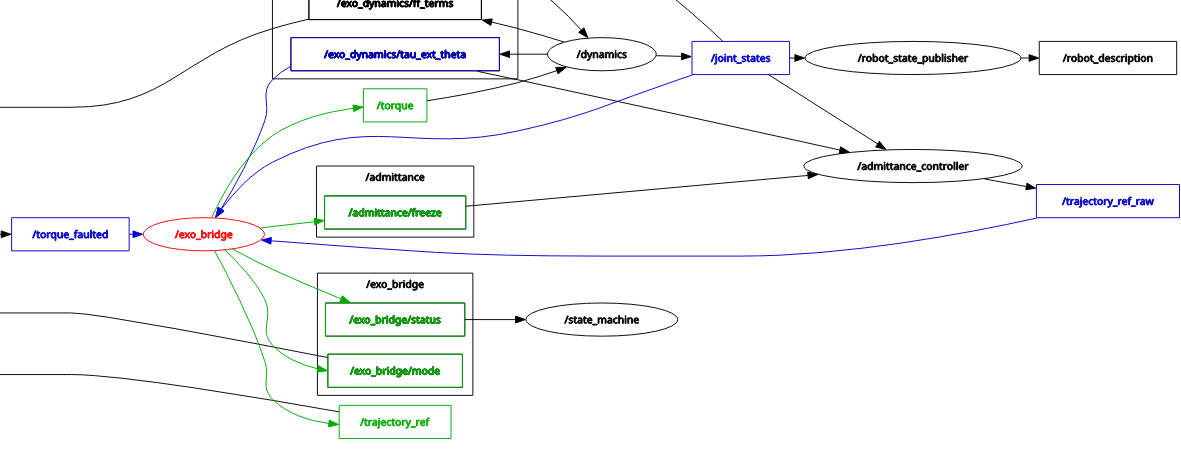
\includegraphics[scale=0.4]{images/chapter5/rosgraph_bridge_evidenziato.png}
    \caption{ROS graph of the Digital Twin with the ExoBridge node highlighted. }
    \label{fig:rosgraph_bridge}
\end{figure}
\FloatBarrier

\subsection{Operating Modes}
The bridge supports four operating modes, each corresponding to a different level of signal intervention. The active mode is set by the state machine plugins through the \textbf{/bridge/set\_mode} service, which accepts a string parameter (\textbf{nominal}, \textbf{compliant}, \textbf{torque\_limit}, or \textbf{stop}). The mode-dependent behavior is implemented in two methods: \textbf{\_safe\_torque()} for the torque channel and \textbf{\_safe\_trajectory\_ref()} for the trajectory reference channel.

\textbf{Nominal mode.} In this mode, all signals pass through the bridge without modification. The torque command from the trajectory controller is forwarded directly to the plant, and the trajectory reference from the admittance controller is forwarded without clamping. This is the mode used during normal rehabilitation operation.

\textbf{Compliant mode.} In this mode, the bridge modifies the trajectory reference to provide a compliant behavior, allowing the plant to move in response to external forces. The trajectory reference is clamped to a symmetric interval around the current joint position, defined by the compliant range parameter. This effectively creates a virtual "cage" around the current position, within which the plant can move freely, but outside of which the trajectory reference is limited. The torque command is also modified by applying a gain reduction factor, which reduces the maximum torque that can be commanded to the plant. This mode allows for safe interaction with the user while still providing some level of assistance.

\textbf{Torque limit mode.} The bridge clamps the torque command to a symmetric interval $[-\tau_{override}, \tau_{override}]$ where $\tau_{override}$ is a configurable parameter. The trajectory reference is not modified in this mode. This mode provides a more restrictive safety envelope than compliant mode, allowing the plant to move freely but limiting the maximum force that can be applied to the user.

\textbf{Stop mode.} This is the most restrictive operating mode, activated upon entry into the \textbf{SAFE\_STOP} state. The bridge performs two simultaneous actions: it commands zero torque to the plant, and it publishes a freeze command on the \textbf{/admittance/freeze} topic to halt the integration of the admittance controller's virtual dynamics. The trajectory reference is replaced by a hold reference at the current crank position with zero velocity and zero acceleration:

\begin{minted}{python}

def _hold_reference(self) -> Optional[Float64MultiArray]:
    theta = self.theta_hold if self.theta_hold is not None \
            else self.get_current_theta()
    if theta is None:
        return copy.deepcopy(self.last_trajectory_ref_in) \
               if self.last_trajectory_ref_in else None
    msg = Float64MultiArray()
    msg.data = [float(theta), 0.0, 0.0]
    return msg

\end{minted}

The hold position $\theta_{hold}$ is captured at the instant the stop mode is activated, ensuring that the reference remains fixed at the last known safe configuration. A configurable
\textbf{stop\_mode parameter} allows selection between \textbf{zero\_torque\_only} (the default, which simply zeros the torque) and \textbf{hold\_only} (which maintains a clamped torque to hold the current position). The \textbf{zero\_torque\_only} strategy is preferred in the current implementation because it guarantees that no force is applied to the user, regardless of the state of the controller or the accuracy of the position measurement.

\subsection{Per-Channel Watchdog}
The bridge implements an independent watchdog system that monitors the \textbf{liveness} of each of the four input channels: \textbf{/torque\_raw}, \textbf{/trajectory\_ref\_raw}, \textbf{/exo\_dynamics/tau\_ext\_theta}, and \textbf{/joint\_states}. Each channel's watchdog tracks the timestamp of the last received message through a dedicated dictionary:

\begin{minted}{python}

self._last_rx: dict[str, Optional[float]] = {
    CH_TORQUE:  None,
    CH_TRAJ:    None,
    CH_TAU_EXT: None,
    CH_JS:      None,
}

\end{minted}

At each iteration of the 200 Hz control loop, the \textbf{\_check\_watchdogs()} method evaluates the age of the most recent message on each channel. If any channel exceeds the configured timeout (default: 0.5 s), or if a channel has never been received after the grace period (default: 2.0 s), the bridge logs the dead channel and issues a safe stop request to the state machine:

\begin{minted}{python}

def _check_watchdogs(self):
    now = self.get_clock().now().nanoseconds * 1e-9
    if (now - self._start_time) < self.watchdog_grace:
        return

    newly_dead = []
    for ch in ALL_CHANNELS:
        last = self._last_rx[ch]
        if last is None:
            if ch not in self._dead_channels:
                newly_dead.append((ch, -1.0))
                self._dead_channels.add(ch)
            continue
        age = now - last
        if age > self.watchdog_timeout:
            if ch not in self._dead_channels:
                newly_dead.append((ch, age))
                self._dead_channels.add(ch)

    if not newly_dead:
        return

    for ch, age in newly_dead:
        self.get_logger().error(
            f'ExoBridge WATCHDOG: channel [{ch}] '
            f'{"never received" if age < 0 else f"dead | age={age:.3f}s"}'
            f' -> SAFE_STOP')

    self._request_safe_stop()

\end{minted}

The \textbf{\_dead\_channels} set ensures that each channel triggers the safe stop request only once: after the initial detection, the channel is marked as dead and subsequent timeout occurrences are suppressed until the channel recovers (i.e., a new message is received). Upon recovery, the channel is removed from the dead set and a log message confirms the restoration. This mechanism prevents repeated safe stop requests for the same channel failure while still detecting new failures on other channels.

The per-channel watchdog operates independently of both the FaultMonitorMode watchdog (which monitors the bridge status topic) and the state machine's bridge liveness check (which monitors the bridge status from the governance layer). This redundancy is deliberate: if the fault monitor crashes, the bridge watchdogs continue to operate; if the bridge's own publishing logic fails, the state machine's liveness check detects the absence of status messages. The three watchdog mechanisms thus form a layered detection network in which no single point of failure can leave the system unmonitored.

\subsection{Bridge Supervision from the State Machine}
In addition to the bridge's own internal watchdogs, the state machine performs two external supervision checks on the bridge at every 10 Hz status publication tick.

\paragraph{Liveness check} The state machine tracks the timestamp of the last received \textbf{/exo\_bridge/status} message. If the elapsed time exceeds the configured \newline \textbf{bridge\_liveness\_timeout} (default: 0.5 s), the bridge is declared dead and a \textbf{SAFE\_STOP} transition is requested:

\begin{minted}{cpp}
void StateMachine::check_bridge_liveness()
{
  const double uptime =
    (this->now() - last_transition_time_).seconds();
  if (uptime < bridge_liveness_grace_ && !bridge_ever_seen_) {
    return;
  }

  if (!bridge_ever_seen_) {
    RCLCPP_ERROR(this->get_logger(),
      "Bridge NEVER seen after %.1fs grace -> SAFE_STOP",
      bridge_liveness_grace_);
    bridge_ever_seen_ = true;
    bridge_alive_ = false;
    request_state_change(
      SafetyState::SAFE_STOP, "bridge_never_seen");
    return;
  }

  const double age =
    (this->now() - last_bridge_status_time_).seconds();

  if (age > bridge_liveness_timeout_) {
    bridge_alive_ = false;
    if (current_state_ == SafetyState::SAFE_STOP) {
      return;
    }
    RCLCPP_ERROR(this->get_logger(),
      "Bridge status TIMEOUT | age=%.3fs > "
      "timeout=%.3fs -> SAFE_STOP",
      age, bridge_liveness_timeout_);
    request_state_change(
      SafetyState::SAFE_STOP, "bridge_liveness_timeout");
  }
}

\end{minted}

The check includes a configurable grace period (default: 3.0 s) during which the bridge is not expected to have published yet, accommodating the startup latency of the supervision node. A special case handles the scenario in which the bridge is never seen at all: after the grace period expires without any status message, the state machine escalates to \textbf{SAFE\_STOP} and sets the \textbf{bridge\_ever\_seen\_} flag to prevent repeated error log entries.

\paragraph{Mode coherence check}  Each bridge status message includes a numeric mode identifier (\textbf{data[7]}) that reflects the bridge's current operating mode. The state machine compares this identifier against the mode expected for the current safety state through the \textbf{expected\_bridge\_mode\_id()} mapping:

\begin{minted}{cpp}

int StateMachine::expected_bridge_mode_id() const
    {
    switch (current_state_) {
        case SafetyState::FAULT_MONITOR:     return 0;
        case SafetyState::TORQUE_LIMIT_MODE: return 1;
        case SafetyState::COMPLIANT_MODE:    return 2;
        case SafetyState::SAFE_STOP:         return 3;
        default: return -1;
        }
    }

\end{minted}

If the reported mode differs from the expected mode, a mismatch counter is incremented. If the counter reaches a configurable threshold (default: 10 consecutive mismatches), the state machine concludes that the bridge has failed to follow a mode change command and escalates to \textbf{SAFE\_STOP}:

\begin{minted}{cpp}

if (bridge_mode_id != expected_id
    && !transition_in_progress_) {
  mode_mismatch_count_++;
  bridge_mode_coherent_ = false;
  if (mode_mismatch_count_ >= mode_mismatch_threshold_) {
    request_state_change(
      SafetyState::SAFE_STOP,
      "bridge_mode_mismatch");
    return;
  }
} else {
  mode_mismatch_count_ = 0;
  bridge_mode_coherent_ = true;
}

\end{minted}

The check is suspended during state transitions (\textbf{transition\_in\_progress\_} flag) and the mismatch counter is reset at every successful transition, because the bridge requires one to two communication cycles to update its mode identifier after receiving a \textbf{set\_mode} command. This tolerance window prevents false positives during the normal transition transient while still detecting genuine mode divergence - for instance, if the /bridge/set\_mode service call fails silently or if the bridge's internal state becomes corrupted.

\subsection{Status Publishing}
The bridge publishes a comprehensive status vector on \textbf{/exo\_bridge/status} at 200 Hz, encoded as a \textbf{Float64MultiArray} with the following layout:

\begin{table}[htbp]
\centering
\small
\caption{Layout of the \texttt{ExoBridge} status message (\texttt{/exo\_bridge/status}).}
\label{tab:bridge_status_layout}
\begin{tabularx}{\textwidth}{c>{\ttfamily}l>{\raggedright\arraybackslash}X}
\toprule
\textbf{Index} & \textnormal{\textbf{Field}} & \textbf{Description} \\
\midrule
0 & is\_stop        & 1.0 if the bridge is in stop mode, 0.0 otherwise \\
1 & is\_limited     & 1.0 if in \texttt{torque\_limit} or \texttt{compliant} mode \\
\addlinespace
2 & theta           & Current crank position from \texttt{/joint\_states} \\
3 & theta\_dot      & Current crank velocity from \texttt{/joint\_states} \\
4 & theta\_hold     & Hold position in stop mode (NaN if not active) \\
\addlinespace
5 & tau\_out        & Torque post-clamp, effectively delivered to the plant \\
6 & tau\_ext\_theta & External force projected onto the crank coordinate \\
\addlinespace
7 & mode\_id        & Numeric mode identifier (0\,=\,nominal, 1\,=\,torque\_limit, 2\,=\,compliant, 3\,=\,stop) \\
8 & tau\_raw        & Torque pre-clamp, as commanded by the trajectory controller \\
\bottomrule
\end{tabularx}
\end{table}

The inclusion of both the pre-clamp (\textbf{tau\_raw}) and post-clamp (\textbf{tau\_out}) torque values is significant for the automatic downgrade mechanism described in Section 5.6. The downgrade logic needs to evaluate whether the fault condition has subsided by examining the torque that the controller \textbf{would like to apply}, not the torque that is actually reaching the plant. If only the post-clamp value were available, the controller output would always appear to be within limits - precisely because the bridge is clamping it - and the downgrade condition would never be satisfied.





\section{Automatic Downgrade}
The escalation mechanisms described in the preceding sections move the system toward progressively more restrictive safety states in response to detected anomalies. An equally important - and considerably more delicate - aspect of the safety architecture is the reverse process: returning the system to a less restrictive state once the fault condition has subsided. This section describes the automatic downgrade mechanism implemented in the state machine, which provides a controlled and conservative path for de-escalation without requiring manual operator intervention.

\subsection{Design Rationale}
In many practical scenarios, particularly during the early stages of Digital Twin development and parameter tuning, fault conditions may be transient in nature. A brief torque spike caused by an aggressive controller gain, a momentary velocity overshoot during a rapid reference change, or a short-lived numerical artifact in the kinematic closure solver can all trigger an escalation to \textbf{COMPLIANT\_MODE} or \textbf{TORQUE\_LIMIT\_MODE}. If the system were to remain in the degraded state indefinitely after such a transient, the operator would need to manually reset it for every occurrence, significantly disrupting the development workflow.

The \textbf{automatic downgrade} addresses this by monitoring the system signals while in a degraded state and progressively accumulating evidence that the fault condition has resolved. Only after a sustained period of nominal behavior - configurable through the \textbf{downgrade\_count\_threshold} parameter - does the state machine autonomously transition to a less restrictive state. The mechanism is disabled by default (\textbf{enable\_automatic\_downgrade: false} in \textbf{safety\_params.yaml}) and is intended for use only when the operator has determined that the predominant fault mode is transient. For persistent or safety-critical faults, manual de-escalation through the ROS 2 service interface remains the recommended approach.

It is important to note that the automatic downgrade never applies to the latched \textbf{SAFE\_STOP} state. A latched safe stop can only be cleared through the explicit \textbf{/reset\_safety\_request} service, regardless of the downgrade configuration. This ensures that the most critical protective action always requires human confirmation.

\subsection{Counter-Based Progressive De-Escalation}
The downgrade logic is evaluated inside the \textbf{bridge\_status\_callback()} of the state machine, at every reception of a bridge status message (200 Hz). Two independent counters track the de-escalation progress for the two degraded states: \textbf{counter\_exit\_torque\_limit\_} and \textbf{counter\_exit\_compliant\_}.

At each cycle, the current torque and velocity values are compared against the corresponding exit thresholds. If both signals are below their respective thresholds, the counter is incremented by one; if either signal exceeds its threshold, the counter is decremented by a configurable negative weight:

\begin{minted}{python}

// From TORQUE_LIMIT_MODE
const bool positive =
  (abs_tau < tau_torque_limit_exit_) &&
  (abs_vel < vel_torque_limit_exit_);

if (positive) {
  counter_exit_torque_limit_ = std::min(
    counter_exit_torque_limit_ + 1,
    downgrade_count_threshold_);
} else {
  counter_exit_torque_limit_ = std::max(
    counter_exit_torque_limit_ - downgrade_negative_weight_,
    0);
}

\end{minted}

The \textbf{asymmetric weighting} is a deliberate design choice. With the default negative weight of 5, a single sample that exceeds the exit threshold erases the progress of five nominal samples. This means that the counter can only advance toward the threshold if at least approximately 83\% of the samples within the observation window are nominal. The asymmetry implements a conservative policy: transient returns to the fault condition are heavily penalized, ensuring that the downgrade only occurs when there is strong statistical evidence of sustained nominal behavior.

The counter is clamped to the interval $[0, downgrade\_count\_threshold]$ to prevent unbounded accumulation in either direction. With the default threshold of 2000 samples at 200 Hz, the minimum time required for a downgrade - assuming perfectly nominal behavior - is 10 seconds. In practice, any intermittent threshold violations extend this duration significantly due to the negative weighting.

\subsection{Transition Paths}
When a downgrade counter reaches its threshold, the state machine evaluates which target state is appropriate. The logic depends on the current state.

From \textbf{TORQUE\_LIMIT\_MODE}, two outcomes are possible. If, at the moment the counter reaches the threshold, both the torque and velocity are also below the stricter compliant exit thresholds, the system transitions directly to \textbf{FAULT\_MONITOR}, bypassing \textbf{COMPLIANT\_MODE} entirely. Otherwise, the system transitions to \textbf{COMPLIANT\_MODE} as an intermediate step:

\begin{minted}{python}

if (counter_exit_torque_limit_ >= downgrade_count_threshold_) {
  counter_exit_torque_limit_ = 0;
  counter_exit_compliant_    = 0;

  if (abs_tau < tau_compliant_exit_
      && abs_vel < vel_compliant_exit_) {
    fault_present_ = false;
    request_state_change(
      SafetyState::FAULT_MONITOR,
      "downgrade_torque_limit_to_nominal");
  } else {
    request_state_change(
      SafetyState::COMPLIANT_MODE,
      "downgrade_torque_limit_to_compliant");
  }
}

\end{minted}

From \textbf{COMPLIANT\_MODE}, the only downgrade target is \textbf{FAULT\_MONITOR}. When the compliant exit counter reaches its threshold, the \textbf{fault\_present\_} flag is cleared and the system returns to nominal operation:

\begin{minted}{cpp}

if (counter_exit_compliant_ >= downgrade_count_threshold_) {
  counter_exit_compliant_ = 0;
  fault_present_ = false;
  request_state_change(
    SafetyState::FAULT_MONITOR,
    "downgrade_compliant_to_nominal");
}

\end{minted}

Both counters are reset to zero after any downgrade transition, ensuring that the observation window restarts from scratch if the system is subsequently re-escalated.

\subsection{Use of Pre-Clamp Torque}
A subtle but critical aspect of the downgrade evaluation concerns the torque signal used for the threshold comparison. As noted in Section 5.5.5, the bridge status vector includes both the post-clamp torque (\textbf{tau\_out}, index 5) and the pre-clamp torque (\textbf{tau\_raw}, index 8). The downgrade logic evaluates the post-clamp torque (data[5]), which represents the torque effectively delivered to the plant.

At first glance, this might seem contradictory: since the bridge is actively clamping the torque in degraded modes, the post-clamp value will always be within limits by construction. However, this is precisely the intended behavior. The downgrade thresholds ($\tau_{compliant\_exit}$ and $\tau_{torque\_limit\_exit}$) are set to values that are safely below the clamp limits, creating a "buffer zone" that the controller must return to before a downgrade can occur. By evaluating the post-clamp torque, the downgrade logic effectively checks whether the controller's output has returned to a safe level, rather than just whether the bridge is successfully clamping it. This ensures that the downgrade reflects a genuine resolution of the fault condition at the controller level, rather than just a temporary mitigation by the bridge.

The pre-clamp torque (\textbf{tau\_raw}) is nonetheless published in the status vector for diagnostic purposes and could be used in alternative downgrade strategies in future iterations of the system.

\subsection{Diagnostic Logging}
To facilitate monitoring and debugging, the downgrade logic emits periodic log messages reporting the progress of the active counter. A message is logged every 200 samples (i.e., once per second at 200 Hz), indicating the current counter value, the threshold, and the percentage of completion:

\begin{minted}{cpp}

    if (counter_exit_torque_limit_ % 200 == 0 &&
    counter_exit_torque_limit_ > 0) {
  RCLCPP_INFO(this->get_logger(),
    "Downgrade progress [TORQUE_LIMIT]: %d/%d (%.1f%%)",
    counter_exit_torque_limit_,
    downgrade_count_threshold_,
    100.0 * counter_exit_torque_limit_
          / downgrade_count_threshold_);
}

\end{minted}

The same progress information is also published as part of the SafetyStatus message (fields downgrade\_progress\_compliant and downgrade\_progress\_torque\_limit), enabling real-time visualization in a GUI or logging infrastructure without relying on console output.

This diagnostic information was already visible in the image 5.1.



\section{Custom Safety Messages}
The communication between the safety nodes relies on a combination of standard ROS 2 service types (std\_srvs/SetBool, std\_srvs/Trigger) and two custom interface definitions provided by the exoskeletron\_safety\_msgs package. These custom definitions were introduced to satisfy two requirements that could not be adequately addressed by the standard ROS 2 message catalog: the need for a structured, multi-field diagnostic status that captures the full internal state of the safety subsystem, and the need for a string-typed service request for mode selection on the bridge.

\subsection{SafetyStatus Message}
The SafetyStatus message is the primary diagnostic output of the state machine, published at 10 Hz on the /safety\_manager/status topic. It consolidates in a single, self-contained message all the information that a supervision system, a logging infrastructure, or a graphical user interface would need to assess the health and operating condition of the safety subsystem. The full message definition is as follows:

\begin{minted}{yaml}

    builtin_interfaces/Time stamp

    string  state
    int32   state_id

    bool    safe_stop_latched
    bool    fault_present
    string  last_fault_reason

    bool    automatic_downgrade_enabled

    int32   counter_exit_compliant
    int32   counter_exit_torque_limit
    int32   downgrade_threshold
    float64 downgrade_progress_compliant
    float64 downgrade_progress_torque_limit

    bool    bridge_alive
    bool    bridge_mode_coherent

    builtin_interfaces/Time last_transition_time
    string  last_transition_reason

\end{minted}

The message is organized into four logical groups. The first group identifies the current safety state, both as a human-readable string (state) and as a numeric identifier (\textbf{state\_id}: 0 for FAULT\_MONITOR, 1 for COMPLIANT\_MODE, 2 for TORQUE\_LIMIT\_MODE, 3 for SAFE\_STOP). The numeric identifier is provided for efficient programmatic consumption, while the string representation facilitates debugging and log analysis.

The second group reports the fault status: whether the SAFE\_STOP latch is active, whether a fault condition is currently present, and the human-readable reason for the last detected fault. The \textbf{last\_fault\_reason} field is particularly useful for post-incident analysis, as it records the specific trigger - such as \newline "\textbf{bridge\_liveness\_timeout}", "\textbf{bridge\_mode\_mismatch}", or \newline"\textbf{safe\_stop\_request}" - that caused the escalation.

The third group provides the downgrade progress information.\newline The \textbf{automatic\_downgrade\_enabled} flag indicates whether the downgrade mechanism is active; if it is not, the remaining fields in this group should be ignored. When active, the counter values, the threshold, and the percentage progress for each degraded state allow an operator or a GUI to monitor how close the system is to an autonomous de-escalation.

The fourth group reports the bridge supervision diagnostics: \textbf{bridge\_alive} indicates whether the bridge status messages are being received within the liveness timeout, and \textbf{bridge\_mode\_coherent} indicates whether the bridge's reported operating mode matches the mode expected by the state machine. Together with the \textbf{last\_transition\_time} and \textbf{last\_transition\_reason} fields, these diagnostics provide a complete snapshot of the safety subsystem state at every publication tick.

\subsection{SetMode Service}
The \textbf{SetMode} service defines the interface through which the state machine plugins command the operating mode of the \textbf{ExoBridge}. Its definition is minimal:

\begin{minted}{yaml}

string mode
---
bool success
string message

\end{minted}

The request contains a single string field specifying the desired mode ("nominal", "compliant", "torque\_limit", or "stop"). The response indicates whether the bridge accepted the mode change and provides a descriptive message in case of rejection - for instance, if an unrecognized mode string is provided. The use of a string-typed mode selector, rather than a numeric enumeration, was chosen for readability and ease of use in command-line testing:

\begin{minted}{bash}

    ros2 service call /bridge/set_mode \
            exoskeletron_safety_msgs/srv/SetMode "{mode: 'stop'}"

\end{minted}

The service is advertised by the \textbf{ExoBridge} node and consumed by the \textbf{BridgeModeClient} base class inherited by each safety mode plugin. As discussed in Section 5.2.2, the client includes response verification logic that logs whether the mode change was confirmed or rejected, providing an auditable trace of all mode transitions commanded by the safety subsystem.




\section{Fault Injection Framework}
The safety mechanisms described in the preceding sections are designed to detect and mitigate fault conditions. However, the correctness and effectiveness of these mechanisms can only be verified by systematically subjecting the system to controlled faults and observing whether the expected protective response is produced. To this end, a dedicated fault injection framework was developed within the \textbf{exoskeletron\_faults} package, providing the ability to introduce realistic, reproducible, and runtime-configurable fault conditions into the Digital Twin without modifying the source code of any other node.

\subsection{Design Choices}
The fault injection framework is guided by three design choices. First, \textbf{transparency}: in its default state (fault inactive), the injector must be completely transparent to the system, forwarding all signals without any modification. No node in the architecture should be able to distinguish between a system with and without the injector present, unless a fault is actively being injected. Second, \textbf{non-invasiveness}: the injector must be insertable into the architecture through topic remapping alone, without requiring changes to the publishers or subscribers of the existing nodes. Third, \textbf{runtime configurability}: all fault parameters - type, magnitude, target channel - must be modifiable at runtime through the ROS 2 parameter interface, allowing the operator to activate, deactivate, and reconfigure faults without restarting any node.

These principles ensure that the fault injector can be deployed in the Digital Twin launch configuration as an optional component, enabled or disabled through a launch argument, without affecting the behavior of the system when inactive.

\subsection{Proxy Architecture}
The \textbf{FaultInjector} node operates as a \textbf{signal proxy}: it subscribes to the original topic published by a controller or sensor node, optionally applies a fault transformation to the signal, and republishes the result on a separate \textbf{\_faulted} topic. The downstream consumer is then remapped to subscribe to the faulted topic instead of the original. This architecture is illustrated schematically for the torque channel:

\begin{enumerate}
    \item The trajectory controller publishes the torque command on \textbf{/torque} (its original topic).
    \item The fault injector subscribes to \textbf{/torque} and publishes on \textbf{/torque\_faulted}.
    \item The dynamic plant, which normally subscribes to \textbf{/torque}, is remapped to subscribe to \textbf{/torque\_faulted} instead.
\end{enumerate}

\begin{figure}[ht]
    \centering
    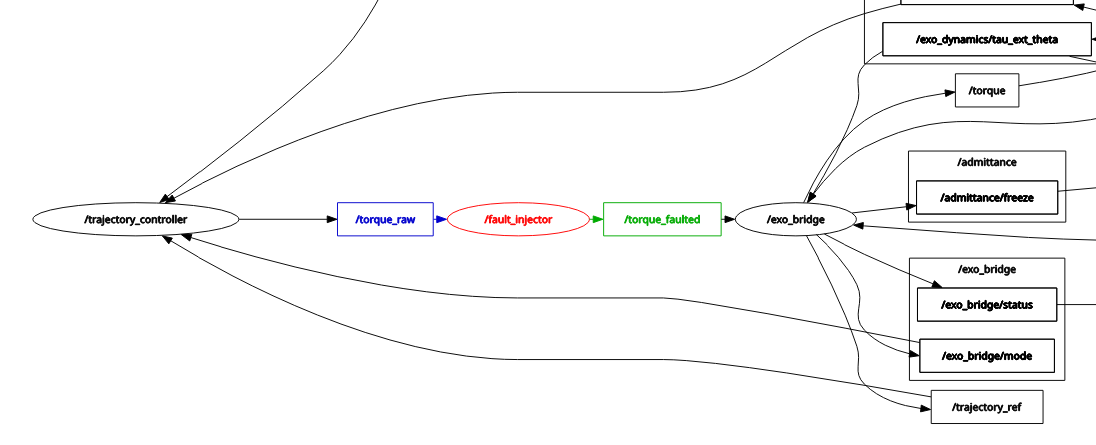
\includegraphics[scale=0.5]{images/chapter5/fault_inj_on_torque.png}
    \caption{Schematic of the fault injection architecture for the torque channel.}
    \label{fig:fault_injection_schema}
\end{figure}
\FloatBarrier


\begin{table}[ht]
\centering
\small
\caption{Supported fault injection channels and their corresponding scenarios.}
\label{tab:fault_scenarios}
\begin{tabularx}{\textwidth}{c>{\ttfamily\raggedright\arraybackslash}p{3cm} l>{\raggedright\arraybackslash}X}
\toprule
\textbf{Ch.} & \textnormal{\textbf{Topic}} & \textbf{Msg Type} & \textbf{Fault Scenario} \\
\midrule
0 & /tau\_ext\_theta  & \texttt{Float64}          & Degraded force sensor, bias in wrench estimation \\
1 & /trajectory\_ref  & \texttt{Float64MultiArray} & Admittance controller fault, corrupted reference \\
2 & /torque           & \texttt{Float64}          & Trajectory controller fault, incorrect motor torque \\
3 & /joint\_states    & \texttt{JointState}       & Encoder fault, position/velocity feedback corruption \\
\bottomrule
\end{tabularx}
\end{table}
\FloatBarrier


\begin{figure}[ht]
    \centering
    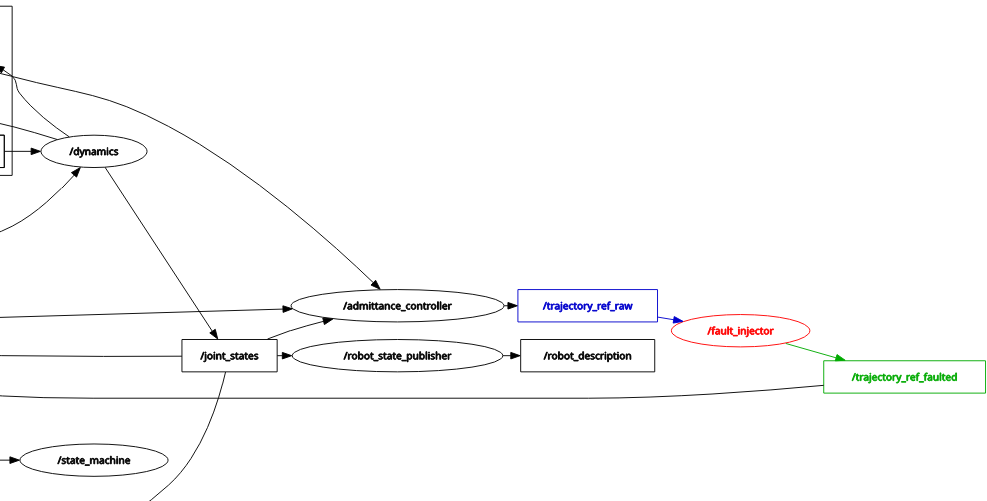
\includegraphics[scale=0.5]{images/chapter5/fault_inj_on_traj_ref.png}
    \caption{Schematic of the fault injection architecture for the trajectory reference channel.}
    \label{fig:fault_injection_schema_2}
\end{figure}
\FloatBarrier


The channel is selected at node startup through the channel parameter and determines which subscriber-publisher pair is instantiated. Channel 3 (\textbf{/joint\_states}) requires special handling because the JointState message contains arrays of values for all joints in the model. The injector identifies the target joint by name (default: rev\_crank) and applies the fault only to the corresponding entry, leaving all other joints unmodified. An additional parameter (\textbf{fault\_js\_field}) selects whether the fault is applied to the position field, the velocity field, or both.

\subsection{Fault Types}
Six fault types are available, each modeling a different class of real-world failure:

\textbf{None}. The signal passes through unmodified. This is functionally equivalent to having the fault inactive, but can be set explicitly as a fault type to distinguish between "injector not armed" (\textbf{fault\_active}: false) and "injector armed but producing no effect" (\textbf{fault\_active}: true, \textbf{fault\_type}: none).

\textbf{Offset}. A constant bias is added to the signal:

\begin{equation}
y(t) = x(t) + m
\end{equation}

where $x(t)$ is the original signal and $m$ is the \textbf{fault\_magnitude} parameter. This models sensor drift, calibration errors, or a persistent estimation bias.

\textbf{Noise}. Gaussian white noise is added to the signal at every sample:

\begin{equation}
    y(t) = x(t) + \mathcal{N}(0, \sigma^2)
\end{equation}

where $\sigma$ is the \textbf{noise\_std} parameter. This models sensor degradation, electromagnetic interference, or quantization noise amplification.

\textbf{Freeze}. The injector stops publishing on the faulted topic entirely. The last received value is stored internally but not forwarded. From the perspective of the downstream consumer, the signal simply ceases to arrive, which is the most realistic model of a crashed or disconnected node. This fault type directly exercises the watchdog mechanisms at both the bridge and state machine levels.

\textbf{Scale}. The signal is multiplied by a configurable factor:

\begin{equation}
    y(t) = x(t) \cdot m
\end{equation}

where $m$ is the \textbf{fault\_magnitude} parameter. This models gain errors, such as an amplifier malfunction or a software bug that causes the controller to produce excessively large or small outputs.

\textbf{Spike}. A single impulse of configurable amplitude and duration is injected:

\begin{equation}
    y(t) = \begin{cases} x(t) + m & \text{if } t \in [t_0,\, t_0 + \Delta t_{\text{spike}}] \\ x(t) & \text{otherwise} \end{cases}
\end{equation}


where $t_0$ is the activation instant and $\Delta t_{\text{spike}}$ is the \textbf{spike\_duration} parameter (default: 50 ms). After the spike expires, the injector returns to transparent operation. This models transient electrical disturbances, single-event upsets, or brief communication glitches.

The fault application logic is centralized in a method, \textbf{\_apply\_fault\_scalar()}, which receives the raw signal value and returns the faulted value. The freeze case is handled separately in the subscriber callbacks, where the publication is suppressed entirely rather than producing a modified value.

\subsection{Runtime Configurability}
All fault parameters are exposed as ROS 2 parameters and can be modified at runtime through the standard parameter interface:

\begin{minted}{bash}

# Arm the injector on channel 2 (torque) with an offset fault
ros2 param set /fault_injector fault_active true
ros2 param set /fault_injector fault_type offset
ros2 param set /fault_injector fault_magnitude 3.0

# Switch to a freeze fault without restarting the node
ros2 param set /fault_injector fault_type freeze

# Deactivate the fault (return to transparent operation)
ros2 param set /fault_injector fault_active false

\end{minted}

Through \textbf{\_current\_fault\_config()}, the parameters are read at every callback invocation ensuring that changes take effect immediately - within one control cycle - without requiring any reconfiguration or restart. Internal transient states (frozen value, spike timing) are automatically reset when the fault type changes, preventing stale state from a previous fault configuration from affecting the new one.

\subsection{Status Publishing}
The fault injector publishes a diagnostic status vector on \textbf{/fault\_injector/status} at a configurable rate (default: 200 Hz), encoded as a Float64MultiArray:

\begin{table}[htbp]
\centering
\small
\caption{Fault injection status message layout (\texttt{/fault\_injector/status}).}
\label{tab:fault_injection_status}
\begin{tabularx}{\textwidth}{cc>{\raggedright\arraybackslash}X}
\toprule
\textbf{Index} & \textbf{Field} & \textbf{Description} \\
\midrule
0 & \texttt{channel}          & Active injection channel (0--3) \\
1 & \texttt{fault\_type\_id}  & Numeric fault type (0\,=\,none, 1\,=\,offset, 2\,=\,noise, 3\,=\,freeze, 4\,=\,scale, 5\,=\,spike) \\
2 & \texttt{fault\_active}    & 1.0 if fault injection is active, 0.0 otherwise \\
3 & \texttt{fault\_magnitude} & Current fault magnitude parameter \\
\addlinespace
4 & \texttt{n\_injections}    & Cumulative number of samples affected by the fault \\
5 & \texttt{last\_raw}        & Last received (pre-fault) signal value \\
6 & \texttt{last\_faulted}    & Last published (post-fault) signal value \\
7 & \texttt{delta}            & Difference between faulted and raw values \\
\bottomrule
\end{tabularx}
\end{table}

This status vector enables real-time monitoring of the injection process and provides the data necessary for post-experiment analysis. The \textbf{delta} field is particularly useful for verifying that the fault is being applied with the expected magnitude, and the \textbf{n\_injections} counter allows the operator to confirm that the fault was active during the intended time window. In combination with the SafetyStatus message from the state machine and the bridge status vector, the injector status provides a \textbf{complete observability chain}: the fault is injected, its effect on the plant signals is recorded, and the safety system's response is documented, all with synchronized timestamps suitable for offline correlation.


\section{Summary}
This chapter has presented the functional safety layer developed for the hand exoskeleton Digital Twin, covering its architecture, individual components, and validation infrastructure.

The safety subsystem is organized into three cooperating layers — enforcement, detection, and governance — each implemented as an independent ROS 2 node or plugin. The \textbf{ExoBridge} enforcement node mediates all control signals between the controllers and the plant, applying mode-dependent torque clamping, velocity limiting, and stop conditions. The \textbf{FaultMonitorMode} plugin continuously evaluates the system signals against configurable thresholds and requests escalation to progressively more restrictive safety states through a debounced, multi-level classification scheme. The \textbf{StateMachine} node governs the overall safety state, enforces a well-defined transition graph with fault latching for the most critical state, and performs external supervision of the bridge through liveness and mode coherence checks.

The separation of concerns between these layers ensures that no single point of failure can leave the system unprotected. The bridge operates autonomously through its per-channel watchdogs even if the state machine becomes unresponsive; the state machine detects the loss of the bridge through its liveness monitor; and the fault monitor provides threshold-based detection that is independent of both the bridge-level watchdogs and the state machine's own supervision logic. This layered redundancy is consistent with the defense-in-depth principle that guided the design.

The automatic downgrade mechanism provides a controlled path for de-escalation from degraded states, using an asymmetrically weighted counter that requires sustained evidence of nominal behavior before permitting a return to less restrictive operation. The mechanism is disabled by default and does not apply to the latched SAFE\_STOP state, preserving the requirement for explicit operator confirmation after critical faults.

The fault injection framework complements the safety architecture by providing a systematic means of introducing controlled, reproducible fault conditions into any of the four critical signal channels. Six fault types — offset, noise, freeze, scale, spike, and none — model a broad range of real-world failure modes, and the runtime configurability of all parameters enables rapid iteration during testing without node restarts.

The functional safety layer described in this chapter operates at the signal and state-machine level, detecting faults through threshold violations and communication watchdogs. A complementary approach, based on a model-based observer that compares the measured system behavior against the predictions of the dynamic model, is briefly discussed in the following chapter. Together, these two detection strategies — threshold-based and model-based — provide overlapping coverage of the fault space, further strengthening the overall safety posture of the Digital Twin.